\documentclass[tikz,border=5pt]{standalone}
\usepackage{amsmath,amssymb,hyperref}
\newcommand{\Spec}{\operatorname{Spec}}
\newcommand{\bT}{\mathbf{T}}
\begin{document}

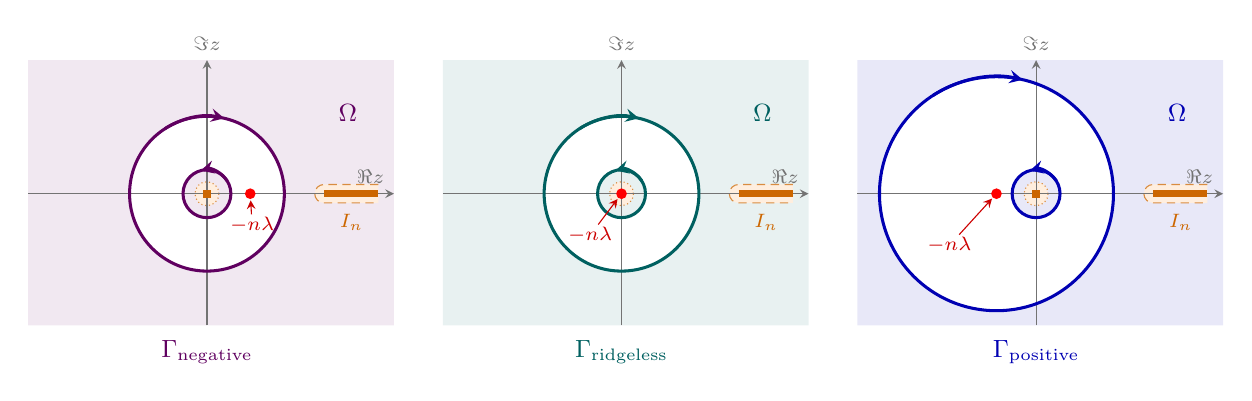
\begin{tikzpicture}[scale=1.17,x=1cm,y=1cm,font=\small,>=stealth]
\colorlet{ridgeorange}{orange!80!black}
\foreach \offset/\shiftcenter/\pole/\name/\ink/\labelx/\labely in {0/0/.47/negative/violet!75!black/.49/-.34,4.50/0/0/ridgeless/teal!75!black/-.34/-.45,9/-.43/-.43/positive/blue!70!black/-.94/-.56}{
  \begin{scope}[xshift=\offset cm]
    \colorlet{ridgecontour}{\ink}
    \pgfmathsetmacro{\outerradius}{.84-\shiftcenter}
    % Omega is the union of the inner disk and the exterior of the outer disk.
    \path[fill=ridgecontour,fill opacity=.09,even odd rule]
      (-1.94,-1.43) rectangle (2.03,1.45) (\shiftcenter,0) circle[radius=\outerradius];
    \fill[ridgecontour,fill opacity=.09] (0,0) circle[radius=.26];
    \fill[orange!13] (1.86,.10)--(1.27,.10) arc[start angle=90,end angle=270,radius=.10]--(1.86,-.10)--cycle;
    \filldraw[fill=orange!13,draw=ridgeorange!75,densely dotted] (0,0) circle[radius=.13];
    \draw[->,black!55] (-1.94,0)--(2.03,0) node[above left,font=\scriptsize] {$\Re z$};
    \draw[->,black!55] (0,-1.43)--(0,1.45) node[above,font=\scriptsize] {$\Im z$};
    \draw[ridgeorange!75,densely dashed] (1.86,.10)--(1.27,.10) arc[start angle=90,end angle=270,radius=.10]--(1.86,-.10);
    \draw[ridgeorange,line width=2.4pt] (1.27,0)--(1.86,0);
    \fill[ridgeorange] (-1.2pt,-1.2pt) rectangle (1.2pt,1.2pt);
    \node[below,text=ridgeorange,font=\scriptsize] at (1.57,-.12) {$I_n$};
    \draw[ridgecontour,line width=1.1pt] (0,0) circle[radius=.26];
    \draw[ridgecontour,line width=1.1pt,->] (32:.26) arc[start angle=32,end angle=105,radius=.26];
    \draw[ridgecontour,line width=1.1pt] (\shiftcenter,0) circle[radius=\outerradius];
    \draw[ridgecontour,line width=1.1pt,->] (\shiftcenter,0) ++(123:\outerradius) arc[start angle=123,end angle=77,radius=\outerradius];
    \node[text=ridgecontour] at (1.53,.88) {$\Omega$};
    \node[font=\scriptsize,text=red!80!black,inner sep=.8pt] (polelabel) at (\labelx,\labely) {$-n\lambda$};
    \draw[->,red!80!black,thin,shorten >=2.4pt] (polelabel)--(\pole,0);
    \fill[red] (\pole,0) circle[radius=1.65pt];
    \node[text=ridgecontour] at (0,-1.72) {$\Gamma_{\mathrm{\name}}$};
  \end{scope}
}
\end{tikzpicture}

\end{document}
